\chapter{МЕТОДЫ УПРАВЛЕНИЯ ЭЛЕКТРОПНЕВМАТИЧЕСКИМ ПРИВОДОМ С ДИСКРЕТНЫМ УПРАВЛЕНИЕМ}\label{ch:ch3}
Управление электропневматическими приводами с дискретными распределителями представляет
собой комплексную задачу, обусловленную нелинейной динамикой пневматических систем и
дискретным характером управляющих воздействий. Эффективное решение данной задачи требует
применения специализированных алгоритмов, способных обеспечить высокую точность позиционирования и
быстродействие системы при ограниченном наборе управляющих состояний. Особый интерес представляет адаптация
классических методов управления к специфике дискретных пневматических систем.

В рамках настоящего исследования рассматривается широкий спектр подходов к управлению электропневматическими
приводами, включающий как современные адаптивные методы, так и модифицированные
классические алгоритмы. Исследуются скользящее управление, прогнозное управление,
нечеткое управление, нейросетевое управление, а также применение широтно-импульсной модуляции (ШИМ)
в сочетании с классическими регуляторами, такими как ПИД-регулятор и его модификации.
Выбор данных методов обусловлен необходимостью комплексного анализа возможностей оптимизации управления
с учетом специфики дискретных пневматических систем. Каждый из рассматриваемых подходов обладает
уникальными преимуществами и ограничениями, детальное изучение которых позволит сформировать
всестороннее представление о перспективах совершенствования алгоритмов управления
электропневматическими приводами с дискретными распределителями.

\section{Анализ режимов работы электропневмопривода}\label{sec:ch3/sec1}

Функционирование электропневмопривода с дискретными распределителями характеризуется конечным
множеством возможных состояний системы, определяемых комбинациями состояний распределителей.
Математически пространство состояний распределителей может быть представлено как:

\begin{equation}\label{eq:state_space}
	\mathbf{U} = \left\{
	[u_1, u_2, u_3, u_4] | u_i \in {0,1}, i = 1,\dots,4
	\right\},
\end{equation}
где $u_i$ -- состояние i-го распределителя (0 - закрыт, 1 - открыт).

Теоретически система, как описано ранее, допускает $2^4 = 16$ различных комбинаций состояний распределителей.
Однако с учетом физических ограничений и требований безопасности целесообразно использование только определенного
подмножества состояний, формирующих основные режимы работы привода.

Классификация этих режимов представлена в следующей таблице \ref{tab:operation_modes}.

\begin{table}[htbp]
	\centering
	\caption{Режимы работы электропневматического привода с дискретными распределителями}
	\label{tab:operation_modes}
	\small
	\begin{tabular}{lcll}
		\midrule
		\textbf{Режим}             & $[u_1,u_2,u_3,u_4]$ & \textbf{Движение} & \textbf{Динамика} \\
		\midrule
		С.П.У.\textsuperscript{1}  & $[1,0,0,1]$         &
		Макс. положит. ускорение   &
		$M\ddot{x} = p_\text{п}F_1 - p_\text{атм}F_2 - R_\text{тр}$                              \\

		У.П.У.\textsuperscript{2}  & $[1,0,0,0]$         &
		Умер. положит. ускорение   &
		$M\ddot{x} = p_\text{п}F_1 - p_2F_2 - R_\text{тр}$                                       \\

		Сл.П.У.\textsuperscript{3} & $[0,0,0,1]$         &
		Мин. положит. ускорение    &
		$M\ddot{x} = p_1F_1 - p_\text{атм}F_2 - R_\text{тр}$                                     \\

		С.О.У.\textsuperscript{4}  & $[0,1,1,0]$         &
		Макс. отриц. ускорение     &
		$M\ddot{x} = p_\text{атм}F_1 - p_\text{п}F_2 - R_\text{тр}$                              \\

		У.О.У.\textsuperscript{5}  & $[0,0,1,0]$         &
		Умер. отриц. ускорение     &
		$M\ddot{x} = p_1F_1 - p_\text{п}F_2 - R_\text{тр}$                                       \\

		Сл.О.У.\textsuperscript{6} & $[0,1,0,0]$         &
		Мин. отриц. ускорение      &
		$M\ddot{x} = p_\text{атм}F_1 - p_2F_2 - R_\text{тр}$                                     \\

		\hline
		Удержание                  & $[0,0,0,0]$         &
		Фиксация положения         &
		$M\ddot{x} = p_1F_1 - p_2F_2 - R_\text{тр}$                                              \\
		\midrule
	\end{tabular}
	\begin{tablenotes}
		\scriptsize
		\item[1] С.П.У. -- сильное положительное ускорение
		\item[2] У.П.У. -- умеренное положительное ускорение
		\item[3] Сл.П.У. -- слабое положительное ускорение
		\item[4] С.О.У. -- сильное отрицательное ускорение
		\item[5] У.О.У. -- умеренное отрицательное ускорение
		\item[6] Сл.О.У. -- слабое отрицательное ускорение
	\end{tablenotes}
\end{table}

Динамическое поведение электропневматического привода для каждого режима может быть
проанализировано как в пространстве давлений, так и в фазовом пространстве
скорость-положение. Векторное поле в фазовом пространстве описывается системой дифференциальных уравнений:

\begin{equation*}
	\begin{cases}
		\dot{x} = v \\
		\dot{v} = \frac{1}{M}(p_1F_1 - p_2F_2 - R_\text{тр}(v))
	\end{cases}
\end{equation*}
где $(x,v)$ -- координаты точки в фазовом пространстве.

Для комплексного понимания динамических процессов в пневмоприводе целесообразно рассмотреть
сравнительные характеристики изменения давлений в полостях пневмоцилиндра
при различных режимах работы, представленные на рисунке \ref{fig:pressure_comparison}.
На графиках отображены процессы для положительного перемещения (выдвижения штока),
поскольку для отрицательного перемещения (втягивания штока) динамика является аналогичной с учетом симметрии системы.

\begin{figure}[htbp]
	\centering
	\includegraphics{part3/pressure_dynamics.pdf}
	\caption{Сравнение динамики установления давлений в различных режимах работы:\\
		а) сильное ускорение; б) умеренное ускорение; в) слабое ускорение; г) режим удержания}
	\label{fig:pressure_comparison}
\end{figure}

Представленные характеристик показывает существенное различие в динамике установления давлений для разных режимов работы.

В режиме сильного положительного ускорения [1,0,0,1] наблюдается максимальный
перепад давлений между полостями цилиндра, что подтверждается системой уравнений:

$$\begin{cases}
		\dot{p}_1 = \frac{\gamma RT_1}{V_1(x)}(G_{1,max} - \frac{p_1}{RT_1}F_1\dot{x}) \\
		\dot{p}_2 = \frac{\gamma RT_2}{V_2(x)}(-G_{4,max} + \frac{p_2}{RT_2}F_2\dot{x})
	\end{cases}$$
где $G_{1,max}$ и $G_{4,max}$ -- максимальные массовые расходы через соответствующие распределители.

Характерной особенностью данного режима является быстрый рост давления $p_1$ до величины, близкой к давлению питания
$p_\text{п}$, с одновременным падением давления $p_2$ до атмосферного давления $p_\text{атм}$. Это обеспечивает интенсивный
разгон штока с последующим выходом на установившуюся скорость, что наглядно демонстрируется на
фазовом портрете (рис. \ref{fig:pp_strong_accelration}). Анализ фазового портрета показывает,
что процесс выхода на установившуюся скорость характеризуется движением изображающей
точки по траектории, асимптотически стремящейся к прямой $v = v_\text{уст}$.

\begin{figure}[htbp]
	\centerfloat{
		\hfill
		\subcaptionbox[List-of-Figures entry]{\label{fig:pp_strong_acceleration_positive}}{
			\includegraphics{part3/pp_strong_acceleration_positive.pdf} }
		\hfill
		\subcaptionbox{\label{fig:pp_strong_acceleration_negative}}{
			\includegraphics{part3/pp_strong_acceleration_negative.pdf} }
	}
	\caption{Фазовые портреты для режима сильного ускорения:\\
		а) положительное ускорение; б) отрицательное ускорение}
	\label{fig:pp_strong_accelration}
\end{figure}

В режимах умеренного ускорения [1,0,0,0]
наблюдается более сложная динамика, обусловленная асимметричным изменением давлений.
При данном режиме динамика давлений описывается системой:

\begin{equation*}
	\begin{cases}
		\dot{p}_1 = \frac{\gamma RT_1}{V_1(x)}(G_{1,max} - \frac{p_1}{RT_1}F_1\dot{x}) \\
		\dot{p}_2 = -\frac{\gamma p_2}{V_2(x)}F_2\dot{x}
	\end{cases}
\end{equation*}

Особенность данного режима заключается в том, что давление в штоковой полости изменяется согласно политропному процессу:

\begin{equation*}
	p_2V_2(x)^n = p_{2,0}V_{2,0}^n = \text{const}
\end{equation*}
где $p_{2,0}$ и $V_{2,0}$ -- начальное давление и объем штоковой полости соответственно в момент запирания полости;
$n$ - показатель политропы.

На фазовых портретах представленных на рисунке \ref{fig:pp_moderate_position_1} и рисунке \ref{fig:pp_moderate_position_2}
отчетливо видно влияние начальных условий на динамику системы. При большем начальном положении штока ($x_0$ равное 0,2~\si{\metre}) наблюдается более
интенсивное торможение вследствие меньшего начального объема запертой полости и, соответственно, более быстрого роста давления при сжатии воздуха.

\begin{figure}[htbp]
	\centerfloat{
		\hfill
		\subcaptionbox[List-of-Figures entry]{\label{fig:pp_medium_acceleration_x_01}}{
			\includegraphics{part3/pp_medium_acceleration_x_01.pdf} }
		\hfill
		\subcaptionbox{\label{fig:pp_medium_acceleration_x_01_scheme}}{
			\raisebox{0.5\height}{\includegraphics{part3/pp_medium_acceleration_x_01_scheme.eps}} }
	}
	\caption{Фазовый портрет и схема пневмоцилиндра при начальном положении штока $x_0 = \num{0.1}$ м ($p_{2,0} = p_\text{атм}$):\\
		а) фазовый портрет; б) схема пневмоцилиндра}
	\label{fig:pp_moderate_position_1}
\end{figure}

\begin{figure}[htbp]
	\centerfloat{
		\hfill
		\subcaptionbox[List-of-Figures entry]{\label{fig:pp_medium_acceleration_x_02}}{
			\includegraphics{part3/pp_medium_acceleration_x_02.pdf} }
		\hfill
		\subcaptionbox{\label{fig:pp_medium_acceleration_x_02_scheme}}{
			\raisebox{0.5\height}{\includegraphics{part3/pp_medium_acceleration_x_02_scheme.eps}} }
	}
	\caption{Фазовый портрет и схема пневмоцилиндра при начальном положении штока $x_0 = \num{0.2}$ м ($p_{2,0} = p_\text{атм}$):\\
		а) фазовый портрет; б) схема пневмоцилиндра}
	\label{fig:pp_moderate_position_2}
\end{figure}

Для более полного понимания влияния начальных условий на динамику системы рассмотрена серия фазовых
портретов при различных комбинациях начального положения штока и давления в запираемой
полости (рис. \ref{fig:pp_moderate_matrix}). Анализ данных портретов демонстрирует, что при
фиксированном начальном положении увеличение давления $p_{2,0}$ приводит к снижению установившейся скорости
движения и увеличению интенсивности торможения. При фиксированном начальном давлении
увеличение координаты $x_0$ вызывает сокращение области достижимых состояний и смещение точки остановки к начальному положению.

\begin{figure}[htbp]
	\centerfloat{
		\hfill
		\subcaptionbox[List-of-Figures entry]{\label{fig:pp_medium_acceleration_x_01_p_2}}{
			\includegraphics{part3/pp_medium_acceleration_x_01_p_2.pdf} }
		\hfill
		\subcaptionbox{\label{fig:pp_medium_acceleration_x_01_p_4}}{
			\includegraphics{part3/pp_medium_acceleration_x_01_p_4.pdf}}
		\hfill
		\subcaptionbox{\label{fig:pp_medium_acceleration_x_02_p_2}}{
			\includegraphics{part3/pp_medium_acceleration_x_02_p_2.pdf}}
		\hfill
		\subcaptionbox{\label{fig:pp_medium_acceleration_x_02_p_3}}{
			\includegraphics{part3/pp_medium_acceleration_x_02_p_4.pdf}}
	}
	\caption{Фазовые портреты при различных начальных условиях: \\
		а) $x_0 = \num{0,1}$ м, $p_{2,0} = 2$ бар; б) $x_0 = \num{0.1}$ м, $p_{2,0} = 4$ бар; \\
		в) $x_0 = \num{0.2}$ м, $p_{2,0} = 2$ бар; г) $x_0 = \num{0.2}$ м, $p_{2,0} = 4$ бар;
	}
	\label{fig:pp_moderate_matrix}
\end{figure}

Математически наблюдаемые эффекты описываются уравнением баланса сил:

\begin{equation*}
	p_\text{п}F_1 - p_{2,0}\left(\frac{V_{2,0}}{V_2(x)}\right)^nF_2 = R_\text{тр}(v),
\end{equation*}
где $V_2(x) = V_{2,0} + A_2(L - x)$ -- текущий объем запертой полости.

Режимы слабого ускорения [0,0,0,1] или [0,1,0,0] характеризуются минимальным перепадом давлений между
полостями пневмоцилиндра. Рассмотрим режим слабого положительного ускорения [0,0,0,1], при котором поршневая полость
изолирована, а штоковая соединена с атмосферой. Динамика давлений в данном режиме описывается системой уравнений:

$$\begin{cases}
		\dot{p}_1 = -\frac{\gamma p_1}{V_1(x)}F_1\dot{x} \\
		\dot{p}_2 = \frac{\gamma RT_2}{V_2(x)}(-G_{4,max} + \frac{p_2}{RT_2}F_2\dot{x})
	\end{cases}$$

На графиках отображенных на рисунке \ref{fig:pressure_comparison} видно, что давление $p_2$ снижается до
тмосферного значения существенно медленнее, чем в режиме сильного ускорения, в то время как
давление $p_1$ изменяется только за счет изменения объема поршневой полости. Данный процесс
характеризуется политропным изменением состояния воздуха в запертой полости:

\begin{equation*}
	p_1V_1(x)^n = p_{1,0}V_{1,0}^n = \text{const}
\end{equation*}
где $p_{1,0}$ и $V_{1,0}$ -- начальные значения давления и объема поршневой полости соответственно.

\begin{figure}[htbp]
	\centerfloat{
		\hfill
		\subcaptionbox[List-of-Figures entry]{\label{fig:pp_weak_acceleration_x01}}{
			\includegraphics{part3/pp_slow_acceleration_x_01_p_3.pdf} }
		\hfill
		\subcaptionbox{\label{fig:pp_weak_acceleration_x02}}{
			\includegraphics{part3/pp_slow_acceleration_x_02_p_3.pdf} }
	}
	\caption{Фазовые портреты для режима слабого ускорения при различных начальных условиях:\\
		а) $x_0 = \num{0.1}$ м, $p_{1,0} = 3$ бар; б) $x_0 = \num{0.2}$ м, $p_{1,0} = 3$ бар}
	\label{fig:pp_weak_acceleration}
\end{figure}

Анализ фазовых портретов представленных на рисунке \ref{fig:pp_weak_acceleration} показывает существенное влияние начального
положения штока на динамику системы. При увеличении начальной координаты $x_0$ наблюдается снижение максимально достижимой
скорости и уменьшение пути перемещения до точки остановки. Это объясняется более быстрым падением давления $p_1$ при расширении
воздуха в запертой полости большего начального объема.

Уравнение баланса сил для данного режима имеет вид:

\begin{equation*}
	p_{1,0}\left(\frac{V_{1,0}}{V_1(x)}\right)^nF_1 - p_\text{атм}F_2 = R_\text{тр}(v)
\end{equation*}

где $V_1(x) = V_{1,0} + A_1x$ - текущий объем поршневой полости.

Характерной особенностью режима слабого ускорения является существенная зависимость динамики
от сил трения. На фазовых портретах это проявляется в виде более крутых траекторий
торможения и меньшей области достижимых состояний по сравнению с режимами сильного и
умеренного ускорения. Данный эффект объясняется тем, что движущая сила, определяемая
разностью давлений в полостях, сопоставима по величине с силами трения.

Для оценки влияния начального давления в запертой полости на динамику системы рассмотрим
серию фазовых портретов при различных значениях $p_{1,0}$ приведенных на рисунке \ref{fig:pp_weak_pressure_matrix}.

\begin{figure}[htbp]
	\centerfloat{
		\hfill
		\subcaptionbox[List-of-Figures entry]{\label{fig:pp_weak_p2}}{
			\includegraphics{part3/pp_slow_acceleration_x_015_p_2.pdf} }
		\hfill
		\subcaptionbox{\label{fig:pp_weak_p3}}{
			\includegraphics{part3/pp_slow_acceleration_x_015_p_3.pdf} }
		\vfill
		\subcaptionbox{\label{fig:pp_weak_p4}}{
			\includegraphics{part3/pp_slow_acceleration_x_015_p_4.pdf} }
	}
	\caption{Фазовые портреты при $x_0 = \num{0.15}$ м и различных начальных давлениях:\\
		а) $p_{1,0} = 2$ бар; б) $p_{1,0} = 3$ бар; в) $p_{1,0} = 4$ бар}
	\label{fig:pp_weak_pressure_matrix}
\end{figure}

Анализ представленных фазовых портретов демонстрирует, что увеличение начального давления $p_{1,0}$ приводит
к возрастанию максимальной скорости движения и увеличению дальности перемещения штока. При этом форма
фазовых траекторий становится более пологой, что свидетельствует о меньшем влиянии сил трения
на динамику системы. Данный эффект объясняется увеличением движущей силы при сохранении характера
её изменения в процессе движения.

%%%%%%%%%%%%%%%%%%%%%%%% mode 0

Режим удержания [0,0,0,0] представляет особый интерес с точки зрения
динамики электропневматического привода, поскольку в данном режиме обе полости
пневмоцилиндра оказываются изолированными.Изменение давлений при этом
происходит исключительно за счет изменения объемов полостей и описывается системой уравнений:

$$\begin{cases}
		\dot{p}_1 = -\frac{\gamma p_1}{V_1(x)}F_1\dot{x} \\
		\dot{p}_2 = -\frac{\gamma p_2}{V_2(x)}F_2\dot{x}
	\end{cases}$$

На графиках изменения давлений, согласно рисунку \ref{fig:pressure_comparison}, наблюдается характерное
политропное изменение состояния воздуха в обеих полостях, описываемое уравнениями:

\begin{equation*}
	\begin{cases}
		p_1V_1(x)^n = p_{1,0}V_{1,0}^n = \text{const} \\
		p_2V_2(x)^n = p_{2,0}V_{2,0}^n = \text{const}
	\end{cases}
\end{equation*}

где $p_{1,0}$, $V_{1,0}$ и $p_{2,0}$, $V_{2,0}$ -- начальные значения давлений и объемов поршневой и штоковой полостей соответственно.

Стабилизация положения штока в режиме удержания обеспечивается преимущественно силами трения, а также дополнительно
поддерживается пневматической жёсткостью, создаваемой сжатым воздухом в изолированных полостях. Баланс сил в данном режиме описывается уравнением:

\begin{equation*}
	p_1F_1 - p_2F_2 = R_\text{тр}(v)
\end{equation*}

\begin{figure}[htbp]
	\centerfloat{
		\hfill
		\subcaptionbox[List-of-Figures entry]{\label{fig:pp_hold_low_pressure}}{
			\includegraphics{part3/pp_hold_low_pressure.pdf} }
		\hfill
		\subcaptionbox{\label{fig:pp_hold_high_pressure}}{
			\includegraphics{part3/pp_hold_high_pressure.pdf} }
	}
	\caption{Фазовые портреты для режима удержания при различных начальных давлениях:\\
		а) низкие начальные давления ($p_{1,0} = 2$ бар, $p_{2,0} = \num{1.8}$ бар);\\
		б) высокие начальные давления ($p_{1,0} = 4$ бар, $p_{2,0} = \num{3.8}$ бар)}
	\label{fig:pp_hold_mode}
\end{figure}

Анализ фазовых портретов для режима удержания показанных на рисунке \ref{fig:pp_hold_mode} показывает высокую эффективность удержания положения штока при различных начальных давлениях.
В системе наблюдается апериодический характер движения с быстрым затуханием скорости, что обусловлено существенным влиянием сил трения.
При этом уровень начальных давлений в полостях оказывает незначительное влияние на характер переходного процесса, что подтверждается схожей формой фазовых траекторий.

\begin{figure}[htbp]
	\centerfloat{
		\hfill
		\subcaptionbox[List-of-Figures entry]{\label{fig:pp_hold_balanced}}{
			\includegraphics{part3/pp_hold_balanced.pdf} }
		\hfill
		\subcaptionbox{\label{fig:pp_hold_unbalanced}}{
			\includegraphics{part3/pp_hold_unbalanced.pdf} }
	}
	\caption{Фазовые портреты при $x_0 = \num{0.15}$ м и различных соотношениях начальных давлений:\\
		а) близкие давления ($p_{1,0} = 3$ бар, $p_{2,0} = 3$ бар);\\
		б) существенная разница ($p_{1,0} = 2$ бар, $p_{2,0} = 4$ бар)}
	\label{fig:pp_hold_matrix}
\end{figure}

Рассмотрение фазовых портретов при различных соотношениях начальных давлений отображенных на  рисунке \ref{fig:pp_hold_matrix} демонстрирует,
что даже при значительной разнице давлений в полостях система сохраняет устойчивое апериодическое движение к положению равновесия.
При близких значениях давлений $p_{1,0}$ и $p_{2,0}$ наблюдается симметричный характер фазовых траекторий. Увеличение разности давлений приводит к незначительной асимметрии траекторий при сохранении общего характера движения.

Математическое описание движения в окрестности положения равновесия может быть получено линеаризацией уравнений движения:

\begin{equation*}
	M\ddot{x} + \left(\frac{\gamma p_{1,0}F_1^2}{V_{1,0}} + \frac{\gamma p_{2,0}F_2^2}{V_{2,0}}\right)x + \nu\dot{x} = 0
\end{equation*}

где $\nu$ -- коэффициент вязкого трения. Существенное преобладание силы трения над пневматической жёсткостью
($\nu \gg \sqrt{M\left(\frac{\gamma p_{1,0}F_1^2}{V_{1,0}} + \frac{\gamma p_{2,0}F_2^2}{V_{2,0}}\right)}$) обуславливает апериодический характер движения системы.

Проведенный анализ режимов работы электропневматического привода с дискретными распределителями
позволил выявить характерные особенности динамики системы для каждого режима функционирования.
В режиме сильного ускорения [1,0,0,1] наблюдается максимальный перепад давлений между полостями и,
как следствие, наибольшая интенсивность разгона штока с последующим выходом на установившуюся скорость.
Режим умеренного ускорения [1,0,0,0] характеризуется существенным влиянием начальных условий на динамику
системы вследствие политропного изменения состояния воздуха в запертой полости. Режим слабого ускорения
[0,0,0,1] демонстрирует значительную зависимость от сил трения при минимальном перепаде давлений между полостями.
Особую роль играет режим удержания [0,0,0,0], в котором стабилизация положения штока обеспечивается преимущественно
силами трения при апериодическом характере затухания скорости. Построенные фазовые портреты и анализ динамики давлений
позволяют обоснованно подходить к выбору режимов работы при проектировании алгоритмов управления электропневматическим
приводом с дискретными распределителями. При этом учет выявленных закономерностей и особенностей каждого режима позволяет
обеспечить требуемые показатели качества позиционирования при минимизации количества переключений распределителей.

\section{ШИМ управление с использование ПИД регулятора}\label{sec:ch3/sec2}

\subsection{Принципы реализации ШИМ в пневматических системах с дискретным управлением}\label{subsec:ch3/sec2/sub1}
Широтно-импульсная модуляция (ШИМ) представляет собой метод формирования квазинепрерывного
управляющего воздействия в системах с дискретными исполнительными элементами.
В контексте пневматических систем с дискретными распределителями применение ШИМ
позволяет преодолеть ограничения, связанные с бинарным характером управления, и обеспечить более
точное регулирование положения и скорости исполнительного механизма.

Механизм формирования квазинепрерывного управляющего воздействия
посредством ШИМ основан на периодическом переключении дискретных
распределителей с определенной частотой и скважностью.

Математически это может быть описано следующим образом:

\begin{equation*}
	u(t) = \begin{cases}
		1, & 0 \leq t < \alpha T \\
		0, & \alpha T \leq t < T
	\end{cases}
\end{equation*}
где $u(t)$ -- управляющий сигнал;
$T$ -- период ШИМ;
$\alpha$ -- коэффициент заполнения $0 \leq \alpha \leq 1$.

На рисунке \ref{fig:ch3:pwm_example} показаны временные диаграммы ШИМ-сигнала
с различными значениями коэффициента заполнения.

\begin{figure}[ht]
	\centerfloat{
		\includegraphics[]{part3/pwm_signal_skewness.pdf}
	}
	\caption{Примеры ШИМ-сигнала с различными значениями коэффициента заполнения:\\ а) $\alpha = \num{0.3}$; б) $\alpha = \num{0.6}$; в) $\alpha = \num{0.9}$}
	\label{fig:ch3:pwm_example}
\end{figure}

Среднее значение управляющего воздействия за период определяется как:
\begin{equation*}
	\bar{u} = \frac{1}{T} \int_0^T u(t) dt = \alpha,
\end{equation*}

Влияние частоты ШИМ на динамику пневмопривода является критическим фактором при
проектировании системы управления. С увеличением частоты ШИМ улучшается
гладкость управляющего воздействия, что способствует снижению пульсаций давления
и повышению точности позиционирования. Однако чрезмерно высокая частота может привести
к повышенному износу распределителей и увеличению энергопотребления.

Для анализа влияния частоты ШИМ на динамику системы может быть использована передаточная функция эквивалентного непрерывного звена:
\begin{equation*}
	W_{\text{ШИМ}}(s) = \frac{1 - e^{-sT}}{sT},
\end{equation*}
где $s$ -- комплексная переменная преобразования Лапласа.
Особенности применения ШИМ для различных типов дискретных
распределителей обусловлены их конструктивными характеристиками и
динамическими свойствами. На рисунке \ref{fig:ch3:pwm_valve_response} показаны
характеристики переходных процессов для распределителей с различным быстродействием.

\begin{figure}[ht]
	\centerfloat{
		\includegraphics[]{part3/pwm_valve_response.pdf}
	}
	\caption{Характеристики переходных процессов для различных типов дискретных распределителей}
	\label{fig:ch3:pwm_valve_response}
\end{figure}

При выборе параметров ШИМ необходимо учитывать соотношение между
периодом ШИМ и динамическими характеристиками распределителя:
\begin{equation*}
	T_{ШИМ} \geq k\tau_{\text{р}},
\end{equation*}
где $\tau_{\text{р}}$ -- время реакции распределителя;
$k$ -- коэффициент запаса (обычно $k \geq 2$).

\subsection{Реализация ПИД-регулирования для пневмоприводов с дискретными распределителями}\label{subsec:ch3/sec2/sub2}
Применение ШИМ в пневмоприводах с дискретными распределителями открывает
возможность использования алгоритмов управления,
изначально разработанных для непрерывных систем.
Одним из наиболее эффективных и широко применяемых методов является
пропорционально-интегрально-дифференциальное (ПИД) регулирование.

Структура ПИД-регулятора для пневмопривода
с дискретными распределителями может быть представлена следующей схемой:
\begin{figure}[ht]
	\centerfloat{
		%    \includegraphics[]{part3/pid_pwn_control.pdf}
		\caption{Структурная схема ПИД-регулятора с ШИМ управлением}
	}
	\label{fig:ch3:pid_pwm_control}
\end{figure}
В данной схеме выходной сигнал ПИД-регулятора преобразуется в коэффициент
заполнения ШИМ, который управляет дискретными распределителями
пневмопривода. Этот подход позволяет достичь высокой точности
управления, характерной для непрерывных систем, в условиях
дискретного исполнительного механизма.

Математическая модель ПИД-регулятора в непрерывной форме описывается уравнением:
\begin{equation}\label{eq:pid_base}
	u_{\text{пид}}(t) = K_{\text{п}} e(t) + K_{\text{и}} \int_0^t e(\tau)d\tau + K_{\text{д}}\frac{de(t)}{dt},
\end{equation}
где
$e(t)$ -- ошибка регулирования;
$K_\text{п}$, $K_\text{и}$, $K_\text{д}$ -- коэффициенты пропорциональной, интегральной и
дифференциальной составляющих соответственно;

Выходной сигнал ПИД-регулятора преобразуется в коэффициент заполнения ШИМ согласно формуле:
\begin{equation*}
	\alpha = \frac{u(i) + u_{max}}{2u_{max}},
\end{equation*}
где $u_{max}$ -- максимальное значение управляющего сигнала.

Однако в рассматриваемой конфигурации ПП с дискретными распределителями
выходной сигнал ПИД-регулятора, как сказано выше, преобразутеся в бинарное
управляющее воздействие посредством ШИМ. При этом возможна только реализация
только двух основных режимов движения: выдвижение штока и его втягивание.

Математически это может быть описано следующим образом:

\begin{equation*}
	\mathbf{u}(t) = \begin{cases}
		[1,0,0,1], & \text{если } u_\text{пид}(t) > 0 \\
		[0,1,1,0], & \text{если } u_\text{пид}(t) < 0
	\end{cases}
\end{equation*}
где $u_\text{пид}(t)$ -- выходной сигнал ПИД-регулятора.

Существенным ограничением данного подхода является отсутствие
прямого управления режимом торможения привода, что может приводить к
перерегулированию и колебательности системы. Выходной сигнал ПИД-регулятора
преобразуется в коэффициент заполнения ШИМ согласно формуле:

\begin{equation*}
	\alpha = \begin{cases}
		\frac{u_\text{ПИД}(t)}{u_{max}},  & \text{если } u_\text{ПИД}(t) > 0 \\
		-\frac{u_\text{ПИД}(t)}{u_{max}}, & \text{если } u_\text{ПИД}(t) < 0
	\end{cases}
\end{equation*}
где $u_{max}$ -- максимальное значение управляющего сигнала.

Данное ограничение является одной из ключевых причин для рассмотрения модифицированных
структур управления, способных обеспечить более эффективное торможение и позиционирование
привода за счет использования дополнительных режимов работы распределителей или реализации
торможения.

\subsection{Модифицированная структура ПИД-регулятора}\label{subsec:ch3/sec2/sub3}

Как было написано выше классическая структура ПИД-регулятора с ШИМ управлением имеет существенные ограничения
в обеспечении эффективного управления электропневматическим приводом с дискретными распределителями.
Основным недостатком является отсутствие прямого управления режимом торможения, что приводит к значительному
перерегулированию и колебательности системы. Для преодоления данных ограничений предлагается модифицированная
структура ПИД-регулятора, обеспечивающая адаптивное торможение на основе анализа динамического состояния системы.

Предложенная модификация базируется на концепции прогнозирования тормозного пути и формировании упреждающего
управляющего воздействия. Математическая модель модифицированного ПИД-регулятора включает три основных
компонента: классический ПИД-регулятор описанный выражением \ref{eq:pid_base}, блок прогнозирования тормозного пути
и блок формирования тормозного воздействия.

Прогнозирование тормозного пути осуществляется на основе анализа
кинетической энергии системы и желаемого ускорения торможения:
\begin{equation*}\label{eq:braking_prediction}
	s_{\text{торм}}(t) = \frac{v(t)|v(t)|}{2a_{\text{торм}}} + \frac{K_{\text{б}}v(t)^2}{2}\text{,}
\end{equation*}
где $v(t)$ -- текущая скорость привода;
$a_{\text{торм}}$ -- желаемое ускорение торможения;
$K_{\text{б}}$ -- коэффициент запаса по тормозному пути, учитывающий инерционность пневматической системы.

Эффективность торможения определяется соотношением между прогнозируемым тормозным путем
и расстоянием до целевой точки. Коэффициент интенсивности торможения вычисляется с использованием нелинейной функции:
\begin{equation*}\label{eq:braking_intensity_expanded}
	k_{\text{торм}}(t) = \begin{cases}
		\left(1 - \min\left(\frac{s_{\text{цель}}(t)}{s_{\text{торм}}(t) \cdot k_{\text{порог}}}, 1\right)\right)^2 \cdot \eta(v), & |v(t)| > v_{\text{порог}}    \\
		0,                                                                                                                         & |v(t)| \leq v_{\text{порог}}
	\end{cases}
\end{equation*}
где $s_{\text{цель}}(t) = |x_{\text{зад}} - x(t)|$ -- расстояние до целевой точки;
$k_{\text{порог}}$ -- пороговый коэффициент начала торможения;
$\eta(v)$ -- функция модуляции интенсивности торможения:
\begin{equation*}\label{eq:modulation_function}
	\eta(v) = 1 - \exp\left(-\left(\frac{|v(t)|}{v_{\text{хар}}}\right)^2\right)\text{,}
\end{equation*}
где $v_{\text{хар}}$ -- характерная скорость, определяющая форму функции модуляции.

Результирующее управляющее воздействие формируется путем комбинации сигналов ПИД-регулятора и тормозного контура:
\begin{equation*}\label{eq:combined_control}
	u_{\text{м}}(t) = (1 - k_{\text{торм}}(t))u_{\text{пид}}(t) + k_{\text{торм}}(t)u_{\text{торм}}(t)\text{,}
\end{equation*}
где $u_{\text{торм}}(t)$ -- сигнал управления в режиме торможения, определяемый направлением движения:
\begin{equation*}\label{eq:braking_control_expanded}
	\mathbf{u}_{\text{торм}}(t) = \begin{cases}
		[0, \alpha{\text{т}}(t), \alpha_{\text{т}}(t), 0],  & v(t) > v_{\text{порог}}      \\
		[\alpha_{\text{т}}(t), 0, 0, \alpha_{\text{т}}(t)], & v(t) < -v_{\text{порог}}     \\
		[0, 0, 0, 0],                                       & |v(t)| \leq v_{\text{порог}}
	\end{cases}
\end{equation*}

Коэффициент заполнения ШИМ в режиме торможения вычисляется с учетом динамических характеристик системы:
\begin{equation*}\label{eq:braking_pwm_expanded}
	\alpha_{\text{т}}(t) = k_{\text{торм}}(t) \cdot \alpha_{\text{макс}} \cdot \left(1 + K_{\text{к}}\frac{d|v(t)|}{dt}\right),
\end{equation*}
где $K_{\text{к}}$ -- коэффициент коррекции, учитывающий скорость изменения модуля скорости.

Для обеспечения численной устойчивости и плавности переключения режимов вводится гистерезисная характеристика активации торможения:
\begin{equation*}\label{eq:hysteresis}
	v_{\text{порог}}(t) = v_{\text{порог}}^0 \cdot \begin{cases}
		1 + \Delta v, & \text{при переходе к торможению} \\
		1 - \Delta v, & \text{при выходе из торможения}
	\end{cases}
\end{equation*}
где $v_{\text{порог}}^0$ -- базовое пороговое значение скорости;
$\Delta v$ -- ширина гистерезиса.

Исследование динамических характеристик системы управления электропневматическим приводом демонстрирует существенные различия
в характере переходных процессов для классической и модифицированной структур ПИД-регулятора с ШИМ.

Для классической структуры характерно наличие значительной колебательности, обусловленной отсутствием эффективного
управления торможением. Это проявляется в перерегулировании при подходе к заданной позиции и возникновении
затухающих колебаний из-за ограниченности режимов работы распределителей.

Модифицированная структура обеспечивает более качественный переходный процесс благодаря
адаптивному торможению и прогнозированию тормозного пути.

\begin{figure}[ht]
	\centerfloat{
		\includegraphics[]{part3/pid_comparison.pdf}
	}
	\caption{Сравнение переходных процессов для классической и модифицированной структуры ПИД-регулятора с ШИМ}
	\label{fig:ch3:transient_comparison}
\end{figure}

Представленные на рисунке \ref{fig:ch3:transient_comparison} результаты наглядно демонстрируют
преимущества модифицированной структуры в обеспечении качества позиционирования электропневматического привода.

% \subsection{Анализ динамических характеристик}\label{subsec:ch3/sec1/sub6}

\section{Управление в скользящих режимах}\label{sec:ch3/sec3}

\subsection{Теоретические основы многорежимного управления в скользящих режимах}\label{subsec:ch3/sec3/sub1}

Метод управления в скользящих режимах представляет собой робастный подход к управлению нелинейными системами,
основанный на переключении структуры управления для обеспечения движения изображающей точки системы вдоль заданной поверхности скольжения в
пространстве состояний. Данный метод особенно эффективен для систем с существенными нелинейностями и неопределенностями, что делает его
перспективным для применения в электропневматических приводах с дискретными распределителями.

Динамика электропневматического привода может быть представлена в виде нелинейной системы дифференциальных уравнений:
\begin{equation*}
\dot{\mathbf{x}} = \mathbf{f}(\mathbf{x}, t) + \mathbf{B}(\mathbf{x})\mathbf{u},
\end{equation*}
где $\mathbf{x} \in \mathbb{R}^n$ -- вектор состояния системы, включающий положение и скорость штока пневмоцилиндра, а также давления в полостях;
$\mathbf{f}(\mathbf{x}, t)$ -- вектор-функция, описывающая естественную динамику системы;
$\mathbf{B}(\mathbf{x})$ -- матрица управления; $\mathbf{u} \in \mathbb{R}^m$ -- вектор управляющих воздействий, соответствующий состояниям дискретных распределителей.

Ключевым элементом метода является определение поверхности скольжения в пространстве состояний, геометрическая интерпретация которой представлена на рисунке~\ref{fig:phase_plane}:
\begin{equation*}
s(\mathbf{x}, t) = 0,
\end{equation*}
где $s(\mathbf{x}, t)$ -- функция переключения.

\begin{figure}[ht]
	\centerfloat{
		\includegraphics[]{part3/phase_plane.eps}
	}
	\caption{Геометрическая интерпретация поверхности скольжения в пространстве состояний}
	\label{fig:phase_plane}
\end{figure}

Для электропневматического привода с позиционным управлением целесообразно использовать функцию переключения вида:

\begin{equation*}
s(\mathbf{x}, t) = \dot{e} + \lambda e + \gamma\int_{0}^{t}e(\tau)d\tau,
\end{equation*}
$\lambda, \gamma$ -- положительные константы, определяющие динамику системы в скольжении.

Как видно из рисунка~\ref{fig:phase_plane}, траектория системы стремится к поверхности скольжения под действием управления,
а затем движется вдоль неё к целевому состоянию. Области притяжения, показанные на рисунке,
обеспечивают сходимость траектории к поверхности скольжения с обеих сторон.

Существование скользящего режима обеспечивается выполнением условия притяжения к поверхности скольжения:
\begin{equation*}
s\dot{s} < 0.
\end{equation*}

Данное условие может быть усилено введением требования η-притяжения:
\begin{equation*}
s\dot{s} \leq -\eta|s|,
\end{equation*}
где $\eta$ -- положительная константа, определяющая скорость сходимости к поверхности скольжения.

В системах с дискретными распределителями управляющее воздействие формируется путем переключения между конечным набором состояний:
\begin{equation*}
\mathbf{u} \in {\mathbf{u}_1, \mathbf{u}_2, ..., \mathbf{u}_k},
\end{equation*}
где $k$ -- количество допустимых комбинаций состояний распределителей. Закон управления принимает вид:

\begin{equation*}
\mathbf{u} = \begin{cases}
\mathbf{u}^+, & s(\mathbf{x}, t) > \varepsilon \\
\mathbf{u}^0, & |s(\mathbf{x}, t)| \leq \varepsilon \\
\mathbf{u}^-, & s(\mathbf{x}, t) < -\varepsilon
\end{cases}
\end{equation*}
где $\varepsilon$ -- ширина зоны гистерезиса, введенная для предотвращения высокочастотных переключений;
$\mathbf{u}^+, \mathbf{u}^0, \mathbf{u}^-$ -- векторы состояний распределителей.

Устойчивость системы может быть исследована с помощью функции Ляпунова:
\begin{equation*}
V = \frac{1}{2}s^2.
\end{equation*}

Условие устойчивости требует:
\begin{equation*}
\dot{V} = s\dot{s} < 0.
\end{equation*}

Характерной проблемой систем со скользящим управлением является возникновение высокочастотных колебаний
(chattering). Для их подавления применяется введение граничного слоя с непрерывной аппроксимацией разрывного управления:
\begin{equation*}
\mathbf{u} = \mathbf{u}^0 - \mathbf{K}\text{sat}\left(\frac{s}{\Phi}\right),
\end{equation*}
где $\Phi$ -- ширина граничного слоя; $\text{sat}(\cdot)$ -- функция насыщения.

Динамическая адаптация ширины зоны гистерезиса может быть реализована согласно выражению:
\begin{equation*}
\varepsilon(t) = \varepsilon_0 + \beta\exp\left(-\alpha\left|\frac{ds}{dt}\right|\right),
\end{equation*}
где $\varepsilon_0$ -- минимальная ширина зоны; $\alpha, \beta$ -- параметры адаптации.

Важным преимуществом скользящего управления является его робастность к
параметрическим возмущениям. При наличии неопределенностей в модели системы:
\begin{equation*}
\mathbf{f}(\mathbf{x}, t) = \mathbf{f}_0(\mathbf{x}, t) + \Delta\mathbf{f}(\mathbf{x}, t),
\end{equation*}
где $\mathbf{f}_0(\mathbf{x}, t)$ -- номинальная модель;
$\Delta\mathbf{f}(\mathbf{x}, t)$ -- ограниченная неопределенность:

\begin{equation*}
|\Delta\mathbf{f}(\mathbf{x}, t)| \leq F_m(\mathbf{x}, t)
\end{equation*}

При соответствующем выборе параметров управления система сохраняет устойчивость и обеспечивает требуемое качество управления.

\subsection{Многорежимное управление в скользящих режимах}\label{subsec:ch3/sec3/sub2}

Анализ динамики электропневматического привода с дискретными распределителями требует
систематического исследования поведения системы при различных конфигурациях поверхностей
скольжения. Рассмотрим математическое описание и особенности формирования управляющих
воздействий для каждой конфигурации, основываясь на результатах анализа режимов, представленных в разделе \ref{sec:ch3/sec1}.

В случае трехрежимного управления закон переключения может быть представлен в следующем виде:
\begin{equation}
\mathbf{u}(s) = \begin{cases}
[1,0,0,1], & s > \varepsilon \\
[0,0,0,0], & |s| \leq \varepsilon \\
[0,1,1,0], & s < -\varepsilon
\end{cases}
\end{equation}
где $\varepsilon$ -- параметр, определяющий ширину зоны переключения, $s$ - функция переключения, определяемая как:

Для данного случая функция переключения имеет вид:
\begin{equation*}
s = \dot{e} + \lambda e
\end{equation*}
где $\lambda$ -- положительный коэффициент.

В фазовом пространстве векторное поле системы разделяется на три области линией
переключения $s = 0$. На рисунке \ref{fig:vector_field_linear} представлено
распределение векторного поля, где в области $s > \varepsilon$ векторы
скоростей направлены к линии переключения под действием
управления $\mathbf{u} = [1,0,0,1]$, соответствующего максимальному ускорению в положительном
направлении. При $s < -\varepsilon$ управление $\mathbf{u} = [0,1,1,0]$ формирует
векторное поле, обеспечивающее движение к линии переключения с противоположной
стороны. В зоне $|s| \leq \varepsilon$ все распределители закрыты $\mathbf{u} = [0,0,0,0]$,
что приводит к замедлению движения за счет сил трения и пневматической жесткости.
\begin{figure}[h]
\centering
\includegraphics[]{part3/phase_portrait_3mode.pdf}
\caption{Распределение векторного поля в фазовом пространстве для линейной поверхности первого порядка}
\label{fig:vector_field_linear}
\end{figure}

При малых значениях параметра $\varepsilon$ возникает эффект <<дребезга>> (chattering),
обусловленный конечным быстродействием электромагнитных распределителей,
инерционностью термодинамических процессов и задержками в системе управления.
Математически эффект <<дребезга>> проявляется в высокочастотных осцилляциях функции
переключения, что может быть выражено соотношением:

\begin{equation*}
\lim_{t \to \infty} \frac{1}{T}\int_t^{t+T} |s(\tau)| d\tau > 0,
\end{equation*}
где $T$ - период осцилляций.

На рисунке \ref{fig:ch3:transient_comparison_linear_mode3} представлены результаты моделирования
для двух значений границы коридора: $\varepsilon = 0,2$ и $\varepsilon = 0,02$.

\begin{figure}[h]
\centering
\includegraphics[]{part3/sliding_mode_linear_transients.pdf}
\caption{Переходные процессы для 3 режимов управления с линейной поверхностью первого порядка:
а) $\varepsilon = 0,2$; б) $\varepsilon = 0,02$}
\label{fig:ch3:transient_comparison_linear_mode3}
\end{figure}

Увеличение параметра $\varepsilon$ позволяет стабилизировать процесс, однако приводит к
росту статической ошибки позиционирования, ограниченной соотношением:

\begin{equation*}
|e_{ss}| \leq \frac{\varepsilon}{\lambda}
\end{equation*}

Для преодоления указанных ограничений предлагается использование многорежимного управления
с пятью или семью режимами, обеспечивающего более гибкое управление торможением
перед достижением целевого положения. При пятирежимном управлении закон управления имеет вид:

\begin{equation}\label{eq:control_law_5_mode}
\mathbf{u}(s) = \begin{cases}
[1,0,0,1], & s > \varepsilon_2 \\
[1,0,0,0], & \varepsilon_1 < s \leq \varepsilon_2 \\
[0,0,0,0], & |s| \leq \varepsilon_1 \\
[0,0,1,0], & -\varepsilon_2 < s \leq -\varepsilon_1 \\
[0,1,1,0], & s \leq -\varepsilon_2
\end{cases}
\end{equation}
где $\varepsilon_1$, $\varepsilon_2$ -- параметры, определяющие границы зон переключения режимов ($\varepsilon_1 < \varepsilon_2$).

Дальнейшее развитие подхода привело к формированию семирежимного управления с более тонкой градацией торможения:

\begin{equation}\label{eq:control_law_7_mode}
\mathbf{u}(s) = \begin{cases}
[1,0,0,1], & s > \varepsilon_3 \\
[1,0,0,0], & \varepsilon_2 < s \leq \varepsilon_3 \\
[0,0,0,1], & \varepsilon_1 < s \leq \varepsilon_2 \\
[0,0,0,0], & |s| \leq \varepsilon_1 \\
[0,1,0,0], & -\varepsilon_2 < s \leq -\varepsilon_1 \\
[0,0,1,0], & -\varepsilon_3 < s \leq -\varepsilon_2 \\
[0,1,1,0], & s \leq -\varepsilon_3
\end{cases}
\end{equation}
где $\varepsilon_1$, $\varepsilon_2$, $\varepsilon_3$ -- параметры, определяющие границы зон переключения режимов ($\varepsilon_1 < \varepsilon_2 < \varepsilon_3$).

Данные модификации обеспечивают более плавное снижение скорости движения перед включением режима удержания,
существенное уменьшение количества переключений распределителей и повышение точности позиционирования
без увеличения частоты переключений. При этом семирежимное управление позволяет достичь
наиболее точного позиционирования за счет более тонкой градации тормозных режимов.

На рисунах \ref{fig:vector_field_linear_5mode} и \ref{fig:vector_field_linear_7mode} представлены векторные поля 
в фазовом пространстве для пятирежимного и семирежимного управления соответственно.

\begin{figure}[htbp]
\centering
\includegraphics[]{part3/phase_portrait_5mode.pdf}
\caption{Распределение векторного поля в фазовом пространстве для линейной поверхности первого порядка и пятирежимного управления}
\label{fig:vector_field_linear_5mode}
\end{figure}

\begin{figure}[htbp]
\centering
\includegraphics[]{part3/phase_portrait_7mode.pdf}
\caption{Распределение векторного поля в фазовом пространстве для линейной поверхности первого порядка и семирежимного управления}
\label{fig:vector_field_linear_7mode}
\end{figure}

\subsection{Анализ поверхностей скольжения при многорежимном управлении}\label{subsec:ch3/sec3/sub3}

Исследование характера движения системы в фазовом пространстве требует детального рассмотрения математической
структуры и особенностей различных поверхностей скольжения.
Проанализируем три типа поверхностей: линейную, интегральную и терминальную.

Линейная поверхность скольжения описывается выражением:

$$
s_1 = \dot{e} + \lambda_1 e,
$$
где $\lambda_1$ -- положительный коэффициент, определяющий наклон линии переключения в
фазовой плоскости.

Динамика системы в скользящем режиме описывается дифференциальным уравнением первого порядка:
$$
\dot{e} + \lambda_1 e = 0
$$
обеспечивающим экспоненциальную сходимость ошибки к нулю с постоянной
времени $T = 1/\lambda_1$. Особенность данной поверхности заключается в
линейном характере убывания ошибки, что приводит к
относительно медленной сходимости при малых отклонениях от целевого положения.

[Далее идут рисунки фазовых портретов для трехрежимного управления с узким и широким коридором, как в предыдущем варианте]

Интегральная поверхность скольжения задается уравнением:

$$
s_2 = \dot{e} + \lambda_1 e + \lambda_2 \int_0^t e(\tau)d\tau,
$$
где $\lambda_1$, $\lambda_2$ -- положительные коэффициенты.

Динамика ошибки описывается дифференциальным уравнением второго порядка:
$$
\ddot{e} + \lambda_1 \dot{e} + \lambda_2 e = 0,
$$

Характеристическое уравнение:

$$
p^2 + \lambda_1 p + \lambda_2 = 0
$$

определяет характер переходного процесса. При $\lambda_1^2 > 4\lambda_2$ система демонстрирует
апериодический характер движения, при $\lambda_1^2 < 4\lambda_2$ -- колебательный.
Оптимальное соотношение $\lambda_1^2 = 4\lambda_2$ обеспечивает критический апериодический процесс.

[Рисунки фазовых портретов для интегральной поверхности]

Терминальная поверхность скольжения представляется выражением:

$$
s_3 = \dot{e} + \beta |e|^{q/p} \text{sign}(e),
$$

где $p$ и $q$ -- нечетные числа, удовлетворяющие условию $1 < q/p < 2$;
$\beta$ -- положительный коэффициент.

Динамика системы описывается нелинейным дифференциальным уравнением:
$$
\dot{e} = -\beta |e|^{q/p} \text{sign}(e).
$$

Особенность данной поверхности заключается в обеспечении конечного
времени сходимости, которое может быть вычислено аналитически:
$$
T_f = \frac{p}{\beta(p-q)}|e(0)|^{1-q/p}
$$

Показатели степени $p$ и $q$ определяют характер
нелинейности: при $e \to 0$ скорость сходимости
увеличивается из-за того, что $q/p > 1$, что обеспечивает более быстрое достижение
целевого положения по сравнению с линейной поверхностью.

[Рисунки фазовых портретов для терминальной поверхности]

[Продолжение анализа фазовых портретов для каждой конфигурации, как в предыдущем варианте]

Для анализа устойчивости и качества движения вдоль каждой поверхности
скольжения рассмотрим соответствующие функции Ляпунова:
Для линейной поверхности скольжения функция Ляпунова имеет вид:
$$
V_1 = \frac{1}{2}s_1^2.
$$

Производная этой функции вдоль траекторий системы:
$$
\dot{V}_1 = s_1\dot{s}_1 = s_1(\ddot{e} + \lambda_1\dot{e}).
$$

При выполнении условия:
$$
s_1\dot{s}_1 \leq -\eta|s_1|
$$
где $\eta$ -- положительная константа, обеспечивается асимптотическая устойчивость скользящего режима.

Для интегральной поверхности расширенная функция Ляпунова учитывает интегральную составляющую:
$$
V_2 = \frac{1}{2}s_2^2 + \frac{\lambda_2}{2}\left(\int_0^t e(\tau)d\tau\right)^2.
$$
Её производная:
$$
\dot{V}_2 = s_2\dot{s}_2 + \lambda_2\left(\int_0^t e(\tau)d\tau\right)e.
$$
Условие существования устойчивого скользящего режима принимает вид:
$$
\dot{V}_2 \leq -\eta|s_2| - \gamma e^2.
$$
где $\gamma$ -- дополнительная положительная константа, обеспечивающая диссипацию энергии в интегральном канале.

Терминальная поверхность скольжения требует использования однородной функции Ляпунова:
$$
V_3 = \frac{1}{2}s_3^2 + \frac{\beta}{1+q/p}|e|^{1+q/p}.
$$

Производная этой функции:
$$
\dot{V}_3 = s_3\dot{s}_3 + \beta|e|^{q/p}\text{sign}(e)\dot{e}.
$$

Условие устойчивости:
$$
\dot{V}_3 \leq -\alpha_1|s_3| - \alpha_2|e|^{1+q/p},
$$
где $\alpha_1$, $\alpha_2$ -- положительные константы.

При многорежимном управлении переключение между режимами модифицирует
условия устойчивости. Для трехрежимного управления
область устойчивых движений определяется соотношением:
$$
\varepsilon < |s| < \beta_{\text{max}}
$$
где $\beta_{\text{max}}$ -- максимальное допустимое отклонение от поверхности скольжения.

При пятирежимном управлении возникают промежуточные зоны устойчивости:
$$
\begin{cases}
\varepsilon_1 < |s| < \varepsilon_2 & \text{для промежуточных режимов} \\
\varepsilon_2 < |s| < \beta_{\text{max}} & \text{для основных режимов}
\end{cases}
$$

Семирежимное управление формирует наиболее сложную структуру областей устойчивости:
$$
\begin{cases}
\varepsilon_1 < |s| < \varepsilon_2 & \text{для слабых режимов} \\
\varepsilon_2 < |s| < \varepsilon_3 & \text{для средних режимов} \\
\varepsilon_3 < |s| < \beta_{\text{max}} & \text{для сильных режимов}
\end{cases}
$$

Особый интерес представляет анализ поведения системы вблизи поверхности скольжения.
Для линейной поверхности скорость приближения к поверхности постоянна:
$$
\lim_{s_1 \to 0} \frac{\dot{s}_1}{s_1} = -\lambda_1.
$$

Для интегральной поверхности скорость приближения зависит от накопленной ошибки:
$$
\lim_{s_2 \to 0} \frac{\dot{s}_2}{s_2} = -\lambda_1 - \lambda_2\int_0^t e(\tau)d\tau.
$$

Терминальная поверхность обеспечивает переменную скорость приближения:
$$
\lim_{s_3 \to 0} \frac{\dot{s}_3}{s_3} = -\beta|e|^{q/p-1},
$$

что объясняет повышенное быстродействие при малых ошибках.

\section{Нечеткое управление электропневматическим приводом с дискретными распределителями}\label{sec:ch3/sec4}
\subsection{Теоретические основы нечеткого управления пневмоприводом}\label{subsec:ch3/sec4/sub1}

Математический аппарат нечеткой логики для управления электропневматическим приводом
с дискретными распределителями основывается на формализации качественных экспертных знаний
о процессе управления с учетом специфики пневматических систем. Данный подход позволяет эффективно
преобразовывать лингвистические правила управления в конкретные управляющие воздействия на распределители.

В основе математического описания лежит определение нечеткого множества $A$ в
универсальном множестве $X$, характеризуемого
функцией принадлежности, как показано на рисунке \ref{fig:membership_functions}:
\begin{equation*}
\mu_A: X \rightarrow \left[0,1\right].
\end{equation*}

\begin{figure}[ht]
\centering
\includegraphics[]{part3/membership_function.pdf}
\caption{Функция принадлежности нечеткого множества}
\label{fig:membership_functions}
\end{figure}

Для формального описания процесса управления вводится понятие лингвистической переменной,
определяемой кортежем из пяти базовых элементов 
\begin{equation*}
\langle \beta, T(\beta), X, G, M \rangle
\end{equation*}
где $\beta$ -- наименование лингвистической переменной;
$T(\beta)$ -- терм-множество значений, представляющее собой названия нечетких переменных;
$X$ -- универсальное множество, определяющее область значений рассматриваемой переменной;
$G$ -- синтаксические правила, порождающие названия значений лингвистической переменной;
$M$ -- семантические правила, задающие функции принадлежности нечетких термов.

Для описания динамического состояния электропневматического привода
используются две основные лингвистические переменные:
\begin{equation*}
\beta = \left\{\beta_1, \beta_2\right\} = \left\{e, v\right\},
\end{equation*}
где $e$ -- ошибка позиционирования;
$v$ -- скорость РО.

Дополнительно система может быть расширена путем включения информации о
давлениях в полостях пневмоцилиндра $p_1$ и $p_2$, что позволяет повысить
качество управления за счет учета термодинамических процессов.

Для ошибки позиционирования определяется следующая структура:
\begin{equation*}
\beta_1 = \text{<<ошибка позиционирования>>}
\end{equation*}

\begin{equation*}
T(\beta_1) =\begin{cases}
	\text{Отрицательная Большая} \\
	\ldots \\
	\text{Нулевая} \\
	\ldots \\
	\text{Положительная Большая}
\end{cases} 
\end{equation*}
при

\begin{equation*}
X_1 = [-x_{\text{max}}, x_{\text{max}}],
\end{equation*}
где $x_{\text{max}}$ -- максимально возможное отклонение от заданного положения.

Синтаксические правила $G$ в данном случае определяют способы формирования составных термов:
\begin{equation*}
\text{G}: \text{знак} + \text{размер},
\end{equation*}
где <<знак>> $\in$ {Отрицательная, Положительная}; <<размер>> $\in$ {Малая, Средняя, Большая}

Семантические правила $M$ устанавливают соответствие между термами и их функциями принадлежности:
\begin{equation*}
M: T(\beta_1) \rightarrow {\mu_i(x) | x \in X_1}.
\end{equation*}

Аналогично для скорости изменения ошибки:
\begin{equation*}
\beta_2 = \text{<<скорость>>}.
\end{equation*}

\begin{equation*}
	T(\beta_2) =\begin{cases}
		\text{Отрицательная Большая} \\
		\ldots \\
		\text{Нулевая} \\
		\ldots \\
		\text{Положительная Большая}
		\end{cases}
\end{equation*}

\begin{equation*}
X_2 = [-v_{\text{max}}, v_{\text{max}}],
\end{equation*}
где $v_{\text{max}}$ -- максимально допустимая скорость.

На рисунке \ref{fig:linguistic_variable_structure} представлена структура лингвистической переменной
<<ошибка позиционирования>> с
7 термами на универсальном множестве $X$ от $-0,2$ до $0,2$.

\begin{figure}[ht]
\centering
\includegraphics{part3/position_error_membership_functions.pdf}
\caption{Структура лингвистической переменной}
\label{fig:linguistic_variable_structure}
\end{figure}

Для каждого терма лингвистической переменной определяется функция принадлежности,
которая может быть представлена в различных формах,
как показано на рисунке \ref{fig:membership_functions_types}.
Наиболее распространенными являются:

Треугольная функция принадлежности:
\begin{equation*}
\mu_A(x; a, b, c) = \max\left(\min\left(\frac{x-a}{b-a}, \frac{c-x}{c-b}\right), 0\right).
\end{equation*}

Гауссова функция принадлежности:
\begin{equation*}
\mu_A(x; c, \sigma) = \exp\left(-\frac{(x-c)^2}{2\sigma^2}\right).
\end{equation*}

Z-образная функция принадлежности:
\begin{equation*}
\mu_A(x; a, b) = \max\left(\min\left(\frac{x-a}{b-a}, 1\right), 0\right).
\end{equation*}

Трапецеидальная функция принадлежности:
\begin{equation*}
\mu_A(x; a, b, c, d) = \max\left(\min\left(\frac{x-a}{b-a}, 1, \frac{d-x}{d-c}\right), 0\right).
\end{equation*}

\begin{figure}[ht]
\centering
\includegraphics{part3/membership_functions.pdf}
\caption{Типы функций принадлежности:\\
а) треугольная; б) гауссова; в) z-образная; г) трапецеидальная}
\label{fig:membership_functions_types}
\end{figure}

Важным аспектом определения лингвистической переменной является выбор
количества термов и их расположения
на универсальном множестве. При этом должны выполняться условия полноты:

\begin{equation*}
\forall x \in X: \sum_{i=1}^n \mu_i(x) > 0,
\end{equation*}
и непротиворечивости:

\begin{equation}
\forall x \in X: \sum_{i=1}^n \mu_i(x) \leq n,
\end{equation}
где $n$ -- количество термов.

База правил нечеткого вывода формируется на основе экспертных знаний
и представляется в виде продукционных правил согласно выражению \ref{eq:fuzzy_rule}. Такие правила как правило,
можно представить в табличном виде согласно рисунку \ref{fig:fuzzy_rules}:

\begin{equation}\label{eq:fuzzy_rule}
R_i: \text{ЕСЛИ } e \text{ есть } A_i \text{ И } \dot{e} \text{ есть } B_i \text{ ТО } u \text{ есть } C_i
\end{equation}

\begin{figure}[ht]
\centering
\includegraphics[]{part3/rule_base.pdf}
\caption{Примерная матрица правил нечеткого вывода для электропневматического привода}
\label{fig:fuzzy_rules}
\end{figure}

Процесс нечеткого вывода реализуется по алгоритму Мамдани,
этапы которого иллюстрируются на рисунке \ref{fig:fuzzy_inference}:

\begin{figure}[ht]
\centering
\includegraphics{part3/Мамдани.eps}
\caption{Алгоритм Мамдани}
\label{fig:fuzzy_inference}
\end{figure}

Фаззификация входных переменных:
\begin{equation*}
\alpha_{ij} = \mu_{A_i}(e_j).
\end{equation*}

Агрегирование подусловий в правилах:
\begin{equation*}
\alpha_i = \min(\alpha_{i1}, \alpha_{i2}).
\end{equation*}

Активизация подзаключений:
\begin{equation*}
\mu'i(y) = \min(\alpha_i, \mu{C_i}(y)).
\end{equation*}

Аккумуляция заключений:
\begin{equation*}
\mu_\Sigma(y) = \max_{i=1,m}\mu'_i(y).
\end{equation*}

Дефаззификация выходной переменной:
\begin{equation*}
y^* = \frac{\int_Y y\mu_\Sigma(y)dy}{\int_Y \mu_\Sigma(y)dy}.
\end{equation*}


\subsection{Разработка базы правил нечеткого вывода}\label{subsec:ch3/sec4/sub2}
\subsection{Синтез нечеткого регулятора для пневмопривода с дискретными распределителями}\label{subsec:ch3/sec4/sub2}

\section{Прогнозное управление}\label{sec:ch3/sec5}
